% OFDM description
\section{Description of OFDM} 
OFDM stands for \textit{Orthogonal Frequency Division Multiplexing}. It relies on different principles used together to combine advantages.\\
%
\indent The most basic of these principles is the \textit{Frequency Division Multiplexing} and consists of the modulation of several ($N$) signals with sub-carriers that are regularly spaced by $\Delta f$, see \figref{fig:OFDMGenerator}.
%
\begin{figure}[H]
  \centering
  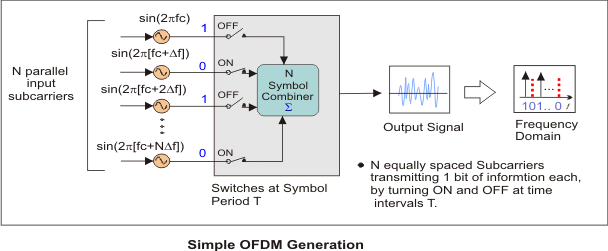
\includegraphics[width=\textwidth]{figures/ofdm-simplegenerator.png}
  \caption{Modulation of signals using OFDM technique \textbf{[source: Keysight]}}
  \label{fig:OFDMGenerator}
\end{figure}
%% TODO : Remove image integrated caption !!
All these modulated signals are then summed into a single signal which is updated periodicly according to the symbol period $T$ and sent through the desired medium.\\
%
\indent The second main concept is the orthogonality of the sub-carriers. When passing to the frequency domain, each sub-carrier will result in a sinc function. Therefore, the spacing, $\Delta f$, between each of them is chosen so that, in frequency domain, each sub-carrier overlap the others orthogonally, which means all the sinc functions have zero crossing and their side-loops cancel each other, while peaks remain distinguishable.
%
\begin{figure}[H]
  \centering
  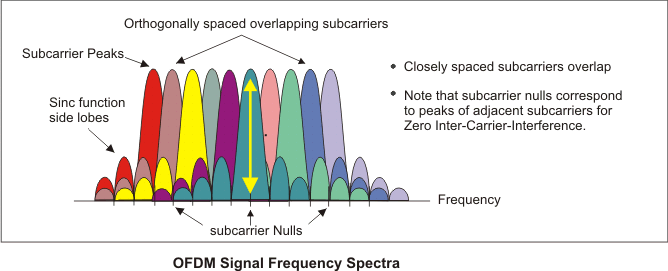
\includegraphics[width=\textwidth]{figures/ofdm-orthogonalspacedsubcarriers.png}
  \caption{Frequency spectrum of OFDM signal \textbf{[source: Keysight]}}
  \label{fig:freqOrthoSinc}
\end{figure}
%
Since, there is no undesirable interference, the spacing between each sub-carrier can be very short. To maintain the orthogonality, this spacing, $\Delta f$, actually has to be the inverse of a symbol period, $T$ :
\begin{flalign}
\eq{\Delta f}{1/T}
\end{flalign}\\
\indent Moreover, by sending information on parallel channels, it is possible to increase the overall data rate and therefore, the spectral efficiency.